\documentclass[12pt]{article}
\usepackage[spanish]{babel}
\usepackage{pgfplots}
\usepackage[utf8]{inputenc}
\usepackage{amsmath,amssymb,amsthm}
\usepackage{graphicx,float}
\usepackage{cancel}
\graphicspath{ {fotos/} }
\providecommand{\abs}[1]{\lvert#1\rvert}
\providecommand{\norm}[1]{\lVert#1\rVert}
\usepackage[a4paper, left=3cm, right=3cm, top=35mm, bottom=20mm]{geometry}
\usepackage{blindtext}

\begin{document}

\bibliographystyle{natbib}

\begin{titlepage}
\begin{center}
{\scshape\huge Física e instrumentación espacial \par}
\vspace{1cm}
{\scshape\Large Cálculo numérico \par}
\vspace{1cm}
{\textbf{{\Huge Resolución Numérica de la Ecuación de Schrödinger}} \par}
\vspace{1.5cm}
{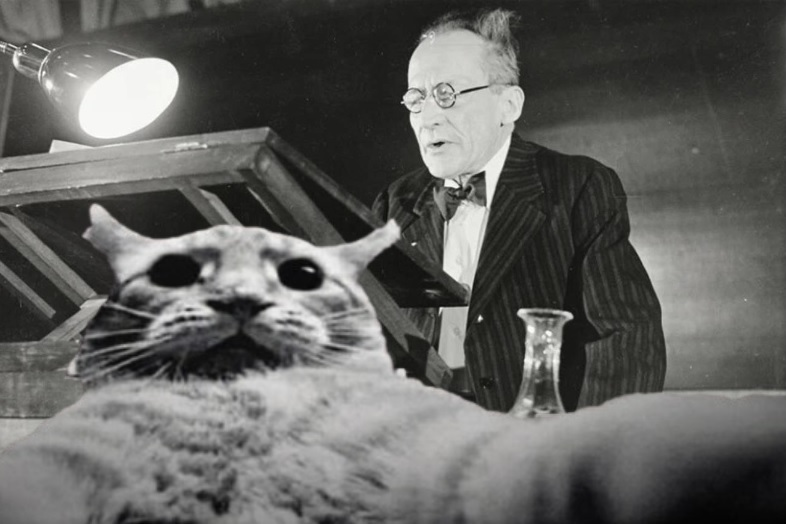
\includegraphics[scale=0.8]{portada}\par}
\vspace{1cm}
{\scshape\Large Abril 2024 \par}
\vspace{1.5cm}
\end{center}
\begin{flushleft}
{\Large Autores: \par}
{\Large 
Víctor Ávila Camargo\\
José Ignacio Miguel Rodríguez\\
Javier Zaragozano Calvo \par
}
\end{flushleft}
\end{titlepage}

\tableofcontents
\newpage	

\section{Introducción}
La ecuación de Schrödinger es una de las ecuaciones más famosas
e importantes de la Física Cuántica. La ecuación de Schrödinger de 1
dimensión en su forma más general es: 
\begin{equation}
i\hbar \frac{\partial}{\partial t}\Psi (x,t)=\hat{H} \Psi (x,t)
\end{equation}
Donde $\hat{H}$ es el Hamiltoniano del sistema. \\
\par
Esta ecuación tiene numerosas variantes. En este artículo, nos 
centraremos en resolver una de sus variantes, la ecuación de Schrödinger
independiente del tiempo que, como su propio nombre indica, el tiempo
no aparece como variable independiente. Esta ecuación se puede obtener a partir de la ecuación descrita arriba, veámoslo.


\subsection{Deducción de la ecuación de Schrödinger independiente del tiempo}
Sea el Hamiltoniano de un sistema cualquiera: 
$\hat{H}=-\frac{\hbar^{2}}{2m}\frac{\partial^{2}}{\partial x^{2}}+V(x,t)$.
Si consideramos que es independiente del tiempo, $V(x,t)$ tiene que ser también 
independiente del tiempo ya que es el único término del Hamiltoniano
con dependencia temporal. Con lo cual $\hat{H}=-\frac{\hbar^{2}}{2m}\frac{\partial^{2}}{\partial x^{2}}+V(x)$ \\
\par
Nuestro objetivo es dejar un lado de la ecuación en función de t y el otro en función de x. Al ser una ecuación diferencial, vamos a usar el método de separación de variables. Entonces: $\Psi (x,t)= g(t) \psi(x)$. 
Y nuestra ecuación queda:
\begin{equation}
i\hbar \psi (x) \frac{d}{d t}g(t)= g(t) \hat{H} \psi (x)
\end{equation}
Como el Hamiltoniano es independiente del tiempo podemos mover libremente 
$g(t)$ porque no va a operar sobre él. Multiplicando ambos 
lados por $\frac{1}{g(t)\psi(x)}$ obtenemos:
\begin{equation}
i\hbar g(t) \frac{d}{d t}g(t)= \psi(x) \hat{H} \psi (x)
\end{equation}
Como cada lado depende de una variable distinta, la igualdad
se cumplirá sí y solo sí el resultado es igual a una constante la cual 
llamaremos E. Entonces por un lado tenemos:

\begin{equation}
\frac{d}{d t}g(t)=-\frac{i}{\hbar} Eg(t)
\end{equation}

Lo que nos da como solución: $g(t)= e^{-\frac{i}{\hbar}Et}$ \\
\par
Por otro lado tenemos:

\begin{equation}
\left(-\frac{\hbar^{2}}{2m}\frac{d^{2}}{d x^{2}}+V(x)\right) \psi(x)=E \psi(x)
\end{equation}

Esta es la ecuación de Schrödinger independiente del tiempo 
y es la que nos centraremos en resolver en este artículo. 
La ecuación se puede abreviar del siguiente modo: $\hat{H} \psi (x)=E \psi (x)$ y vemos
que es una ecuación de autovalores donde $E$ se corresponde con el autovalor
de $\hat{H}$. \\
\par
Sin embargo, resolver esta ecuación no es nada fácil y, 
por ello, será necesario emplear métodos numéricos, 
los cuales serán descritos en detalle 
en las secciones posteriores, para encontrar una solución aproximada. \\
\par 
Una inquietud que le puede surgir al lector es qué interpretación
tiene las soluciones que se obtengan. Así que vamos a intentar esclarecer
esta duda en el siguiente apartado


\subsection{Interpretación de la ecuación de Schrödinger y sus soluciones}
Las soluciones que obtenemos son
funciones de onda que van asociadas a la partícula que queramos 
describir. Esto es debido a la dualidad onda-partícula que caracteriza
a todas las partículas del Universo. Sin embargo, no podemos ver
estas funciones de onda del modo clásico, tenemos que verlas como
funciones de probabilidad que nos indican en qué zonas es más probable que se encuentre la partícula. Esta función de probabilidad
se puede describir como: $dP(x,t)=\left\lvert \Psi (x,t) \right\rvert^{2} dV$.
Esto es la probabilidad de encontrar una partícula en un fragmento
de volumen infinitesimal. Al ser una función de probabilidad cumple que:
$\int_{espacio} \left\lvert \Psi (x,t) \right\rvert^{2} \,d^{3}x=1$. \\
\par
Por otro lado, también encontramos valores de E asociados a la función y al Hamiltoniano. Para ver lo que significan las E que obtenemos, vamos a calcular el valor esperado de $\hat{H}$:
\begin{align}
\langle \hat{H} \rangle_{\Psi (x,t)} \notag 
&=\int \Psi (x,t)^{*} \hat{H} \Psi (x,t) \,dx= \notag \\
&=\int \Psi (x,t)^{*} E \Psi (x,t) \,dx= E
\end{align}
Por definición del valor esperado de $\hat{H}$, sabemos que representa
la  energía total del sistema. Es decir, los autovalores que obtengamos
al resolver la ecuación nos darán un valor para la energía
del sistema. \\
\par
Una vez hechas todas estas aclaraciones introductorias, ya podemos
comenzar con la descripción de todos los métodos numéricos y 
también podemos ver las soluciones obtenidas.

\newpage
\section{Métodos de derivación numérica}
\subsection{Método de las diferencias finitas}
El método de diferencias finitas (FDM) es un método de aproximación para resolver ecuaciones diferenciales, su principio fundamental es transformar una ecuación diferencial en un sistema de ecuaciones algebraicas que podamos resolver. El principio del método de diferencias finitas fue desarrollado por primera vez por el excelentísimo matemático L. Euler (1707-1783), quien en 1768 dio un formato diferencial para problemas unidimensionales. En 1908, C. Runger (1856-1927) extendió el método de la diferencia a problemas bidimensionales. Sin embargo, en aquellos días, convertir la solución de ecuaciones diferenciales en la solución de un gran número de ecuaciones algebraicas era sin duda transformar un problema en otro, por lo que no se usaba ampliamente. Con el desarrollo de la tecnología informática, es posible resolver de forma rápida y precisa enormes ecuaciones algebraicas, por lo que poco a poco se ha ido utilizando ampliamente. 
\\
\\
Este método nos será de gran utilidad ya que si queremos resolver la ecuación de Schrödinger
\begin{equation}\label{eq2}
\frac{\hbar^2}{2m} \frac{\partial^2\psi}{\partial x^2} + V(x)\psi = E \psi
\end{equation}
Nada más y nada menos que en el primer término ya nos encontramos una derivada segunda, lo que convierte nuestro problema en resolver una ecuación diferencial.
Nuestro objetivo será aproximar esta derivada segunda  por el método propuesto para que seamos capaces de computar nuestra ecuación obtener soluciones,
más tarde estudiaremos el impacto de realizar esta aproximación y error que conlleva aplicarla.\\

El método de diferencias finitas consiste en discretizar el espacio en el que estemos trabajando 
y así transformar la distancia infinitesimal entre puntos de las derivadas en una distancia $h$ 
. Por tanto dividimos un intervalo $[a,b]$ donde la función sea continua $N$ veces,
el espacio entre los puntos que nos queden lo llamaremos distancia de paso ($h$) y el tamaño de este nos dará la precisión de nuestra aproximación como veremos más adelante.\\

Este concepto puede hacerse más sencillo de comprender al ver la siguiente figura:


\begin{figure}[H]
\centering
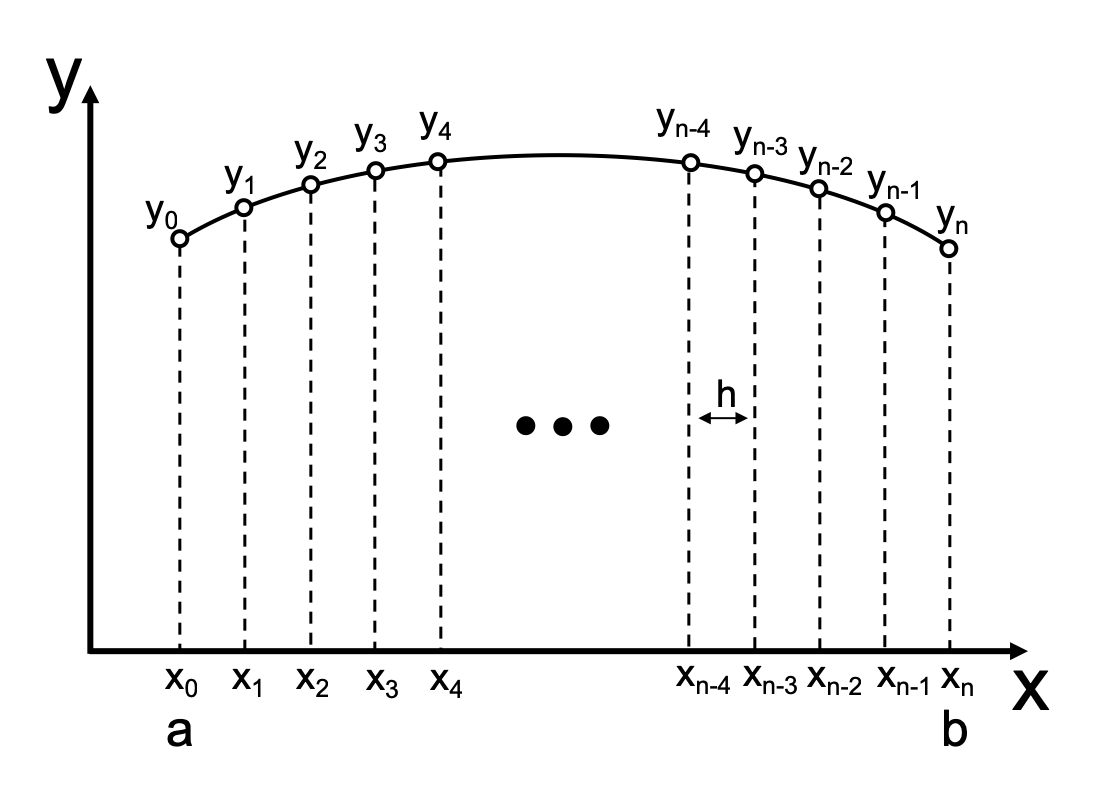
\includegraphics[width=4in]{23.03.01-Finite-difference}
\label{finite_difference}
\end{figure}


\subsubsection{Diferencial de primer orden}

Para obtener una aproximación de la diferenciación en este nuevo espacio lo que nos viene a la mente es la definición de derivada, que la aproximaremos de la siguiente manera:

\begin{equation}\label{eq:eq1}
u'(x)=\lim_{h \to 0}  \frac{u(x+h)-u(x)}{h} \approx \frac{u(x+h)-u(x)}{h}
\end{equation}

\begin{center}
\begin{tikzpicture}[scale=1.1]
\begin{axis}[
axis lines = left,
xlabel = $x$,
ylabel = {$y$},
legend pos=outer north east,
xmin=0, xmax=2,
]
\addplot [
domain=0:10, 
samples=100, 
color=green,
]
{sqrt(x)};
\addlegendentry{$y = u(x)$}

\addplot [
domain=0:10, 
samples=100, 
color=purple,
]
{0.5*x + 0.5};
\addlegendentry{$k_1 = u'(x)$}

\addplot [
domain=0:10, 
samples=100, 
color=blue,
]
{0.449*x + 0.550};
\addlegendentry{$k_f = \frac{u(x+h)-u(x)}{h}$}

\draw[dashed] (axis cs:1,0) -- (axis cs:1,1);
\draw[dashed] (axis cs:1.5,0) -- (axis cs:1.5,1.22);

\end{axis}
\end{tikzpicture}
\end{center}

La recta roja corresponde a la derivada de la función $\sqrt{x}$ en el punto $x=1$,
mientras que la recta azul corresponde a la de nuestra aproximación con paso $h=1$.
Como se puede observar es realmente parecido y según hagamos el paso más pequeño 
esta diferencia se hará menor.\\

Se nos puede ocurrir otra aproximación de la derivada, en vez de aproximarlo con el punto siguiente podríamos tratar de aproximarlo con el punto anterior.\\

\begin{center}
\begin{tikzpicture}[scale=1.1]
\begin{axis}[
axis lines = left,
xlabel = $x$,
ylabel = {$y$},
legend pos=outer north east,
xmin=0, xmax=2,
]
\addplot [
domain=0:10, 
samples=100, 
color=green,
]
{sqrt(x)};
\addlegendentry{$y = u(x)$}

\addplot [
domain=0:10, 
samples=100, 
color=purple,
]
{0.5*x + 0.5};
\addlegendentry{$k_1 = u'(x)$}

\addplot [
domain=0:10, 
samples=100, 
color=brown,
]
{0.5857*x + 0.4142};
\addlegendentry{$k_b = \frac{u(x)-u(x-h)}{h}$}

\draw[dashed] (axis cs:1,0) -- (axis cs:1,1);
\draw[dashed] (axis cs:0.5,0) -- (axis cs:0.5,0.707);

\end{axis}
\end{tikzpicture}
\end{center}

Por lo tanto, aquí primero necesitamos discretizar el dominio de la solución y 
luego obtener la aproximación diferencial en cada punto discreto por separado. 
Para el problema unidimensional divida el intervalo de la solución en partes iguales.\\

La forma discreta de la ecuación (\ref{eq:eq1}) se expresa como: 								
\begin{equation}
u'_i(x)=\frac{1}{h}(u_{i+1} - u_i)
\end{equation}
y la misma, pero utilizando el punto anterior y no el siguiente:
\begin{equation}
u'_i(x)=\frac{1}{h}(u_i-u_{i-1})
\end{equation}
Demostraremos ahora de donde salen estas fórmulas que tan hábilmente se nos han ocurrido.\\

Para la derivada de primer orden si aproximamos por Taylor:

\begin{equation*}
u(x+h)=u(x) + hu'(x)+ \frac{h^2}{2}  u''(x)+ \frac{h^3}{6} u^{(3)}(x+\xi) 
\end{equation*}

donde $\xi\in (0,h)$. La fórmula de la diferencia directa para el diferencial de primer orden se puede obtener deformando la ecuación anterior:

\begin{equation}
u_F'(x)=\frac{u(x+h)-u(x)}{h} - \frac{h^2}{2}u''(x+\xi)
\end{equation}

Ahora si aproximamos por Taylor $u(x-h)$:

\begin{equation*}
u(x-h)=u(x) - hu'(x)+ \frac{h^2}{2}  u''(x) - \frac{h^3}{6} u^{(3)}(x+\xi)
\end{equation*}

donde $\xi\in (0,h)$, si deformamos la ecuación de forma similar al caso anterior obtenemos:

\begin{equation}
u_B'(x)=\frac{u(x)-u(x-h)}{h} + \frac{h^2}{2}u''(x+\xi)
\end{equation}

Si juntamos ambas ecuaciones obtenemos la fórmula de la diferencia central para el diferencial de primer orden

\begin{equation}
u_C'(x)=\frac{u(x+h)-u(x-h)}{2h} - \frac{h^2}{6}u^{(3)}(x+\xi)
\end{equation}

Dado que el error aquí es relativo al tamaño del paso, se puede ver que las fórmulas de la diferencia hacia adelante y hacia atrás tienen una precisión de aproximación de primer orden $O(h)$, mientras que la diferencia central tiene una precisión de aproximación de segundo orden $O(h^2)$, es por esto que nos interesa juntar ambas ecuaciones (cuanto mayor sea el orden, antes tiende el error a cero). Para el caso anterior obtendríamos la siguiente aproximación:\\

\begin{center}
\begin{tikzpicture}[scale=1.1]
\begin{axis}[
axis lines = left,
xlabel = $x$,
ylabel = {$y$},
legend pos=outer north east,
xmin=0, xmax=2,
]
\addplot [
domain=0:10, 
samples=100, 
color=green,
]
{sqrt(x)};
\addlegendentry{$y = u(x)$}

\addplot [
domain=0:10, 
samples=100, 
color=purple,
]
{0.5*x + 0.5};
\addlegendentry{$k_1 = u'(x)$}

\addplot [
domain=0:10, 
samples=100, 
color=red,
]
{0.51763*x + 0.4142};
\addlegendentry{$k_c = \frac{u(x+h)-u(x-h)}{2h}$}

\draw[dashed] (axis cs:1,0) -- (axis cs:1,1);


\end{axis}
\end{tikzpicture}
\end{center}

Vemos como la pendiente de las rectas es mucho más similar que en los casos anteriores, por tanto, es coherente con nuestra demostración sobre la precisión de esta nueva aproximación de la derivada.

\subsubsection{Diferencial de segundo orden}

Para nuestra ecuación, sin embargo, no necesitamos obtener una aproximación de la derivada de primer orden si no de la de segundo orden. Por tanto, trabajaremos ahora con la demostración de esta.\\

Como anteriormente realizamos la expansión de Taylor:

\begin{equation*}
u(x+h)=u(x) + hu'(x)+ \frac{h^2}{2}  u''(x) + \frac{h^3}{6} u^{(3)}(x)+\frac{h^4}{12}u^{(4)}(x+\xi)
\end{equation*}

Pasando el término u''(x) a la derecha obtenemos:
\begin{equation}
u_F''(x)=-\frac{2u(x)}{h^2} - \frac{2u'(x)}{h} - \frac{h}{3}u^{(3)}(x)-\frac{h^2}{6}u^{(4)}(x+\xi) {h^2} + \frac{2u(x+h)}{h^2}
\end{equation}

De igual manera  obtenemos:

\begin{equation*}
u(x-h)=u(x) - hu'(x)+ \frac{h^2}{2}  u''(x) - \frac{h^3}{6} u^{(3)}(x)+\frac{h^4}{12}u^{(4)}(x+\xi)
\end{equation*}

\begin{equation}
u_B''(x)=-\frac{2u(x)}{h^2}  + \frac{2u'(x)}{h} + \frac{h}{3}u^{(3)}(x)-\frac{h^2}{6}u^{(4)}(x+\xi) {h^2} + \frac{2u(x-h)}{h^2}
\end{equation}
Juntando ambas obtenemos:
\begin{eqnarray*}
\frac{1}{2}(-\frac{2u(x)}{h^2} - \bcancel{\frac{2u'(x)}{h}} - \bcancel{\frac{h}{3}u^{(3)}(x)}-\frac{h^2}{6}u^{(4)}(x+\xi) {h^2} + \frac{2u(x+h)}{h^2} -\frac{2u(x)}{h^2} + \\ + \bcancel{\frac{2u'(x)}{h}} +\bcancel{\frac{h}{3}u^{(3)}(x)}-\frac{h^2}{6}u^{(4)}(x+\xi) {h^2} + \frac{2u(x-h)}{h^2}) \rightarrow
\end{eqnarray*}
\begin{equation}
\rightarrow u_C''(x)=\frac{u(x+h)-2u(x)+u(x-h)}{2h^2} - \frac{h^2}{6}u^{(4)}(x+\xi)
\end{equation}

Donde volvemos a apreciar que tenemos una precisión de aproximación de segundo orden relativa al tamaño del paso.

\subsubsection{Error de aproximación en el método de las diferencias finitas}

Si recopilamos los errores de este método de derivación numérica obtenemos:

\begin{flushleft}
-Derivada de primer orden: diferencia ordinaria: 
$E \leq \frac{M_2}{2}h \sim O(h)$\\ donde $M_2 = \smash{\displaystyle\max_{x \in [x_0,x_0+h]}} |f''(x)|$
\end{flushleft}

\begin{flushleft}
-Derivada de primer orden: diferencia central: 
$E \leq \frac{M_3}{6}h^2 \sim O(h^2)$\\ donde $M_3 = \smash{\displaystyle\max_{x \in [x_0-h,x_0+h]}} |f'''(x)|$
\end{flushleft}

\begin{flushleft}
-Derivada de segundo orden: diferencia ordinaria:
$E \leq \frac{M_4}{12}h^2 \sim O(h^2)$\\ donde $M_4 = \smash{\displaystyle\max_{x \in [x_0-h,x_0+h]}} |f^{(4)}(x)|$
\end{flushleft}




\subsection{Aproximación de la ecuación de Schrödinger}
Si ahora aplicamos esto a nuestra ecuación de Schrödinger:
\begin{equation*}
-\frac{\hbar^2}{2m} \frac{\partial^2\psi}{\partial x^2} + V(x)\psi = E \psi
\end{equation*}

Podemos sustituir la derivada segunda por nuestra aproximación, quedando de la siguiente manera:

\begin{equation}
-\frac{\hbar^2}{2m} \frac{\psi_{i+1}(x)-\psi_i(x)+\psi_{i-1}(x)}{h^2} + V_i(x)\psi_i = E \psi_i(x)
\end{equation}

Ahora debemos determinar un intervalo $[a,b]$ que será la región donde resolveremos 
la ecuación. Esta región la dividiremos en N subintervalos, resultando en N+1 puntos y siendo h la distancia entre estos.\\

El valor de la función en $x_0$ y en $x_n$ será 0, ya que la partícula estará confinada en dicho intervalo. Esto será lo que nos dará nuestras condiciones de frontera. Así pues, tendremos que resolver la función en los N-1 puntos restantes.

Nuestra matriz de energía cinética será:

\begin{equation}
T=\frac{-\hbar^2}{2m} \left(
\begin{matrix}
\frac{-2}{h^2} & \frac{1}{h^2} & 0 & 0 &  \cdots & 0 \\
\frac{1}{h^2} & \frac{-2}{h^2} & \frac{1}{h^2} & 0 & \cdots & 0\\
0 & \frac{1}{h^2} & \frac{-2}{h^2} & \frac{1}{h^2} & \cdots & 0\\
\vdots & \vdots&\ddots &\ddots &\ddots& \vdots \\
0 & 0   &\cdots &\frac{1}{h^2}& \frac{-2}{h^2} & \frac{1}{h^2} \\
0 & 0 & 0  &\cdots & \frac{1}{h^2} & \frac{-2}{h^2} \\
\end{matrix}
\right)
\end{equation}

Mientras que la de energía potencial será:

\begin{equation}
V= \left(
\begin{matrix}
V_1 & 0 & 0 & 0 &  \cdots & 0 \\
0 & V_2 & 0 & 0 & \cdots & 0\\
0 & 0 & V_3 & 0 & \cdots & 0\\
\vdots & \vdots&\ddots &\ddots &\ddots& \vdots \\
0 & 0   &\cdots &0& V_{n-1} & 0 \\
0 & 0 & 0  &\cdots & 0 & V_{n} \\
\end{matrix}
\right)
\end{equation}

Construimos nuestra matriz Hamiltoniana de la siguiente forma:
\begin{equation}
H=T+V
\end{equation}
Haciendo esto obtenemos el siguiente sistema lineal: \\

\begin{equation*}
\frac{-\hbar^2}{2m} \left(
\begin{matrix}
\frac{-2}{h^2} & \frac{1}{h^2} & 0 & 0 &  \cdots & 0 \\
\frac{1}{h^2} &  \frac{-2}{h^2} & \frac{1}{h^2} & 0 & \cdots & 0\\
0 & \frac{1}{h^2} &  \frac{-2}{h^2} & \frac{1}{h^2} & \cdots & 0\\
\vdots & \vdots&\ddots &\ddots &\ddots& \vdots \\
0 & 0   &\cdots &\frac{1}{h^2}&  \frac{-2}{h^2} & \frac{1}{h^2} \\
0 & 0 & 0  &\cdots & \frac{1}{h^2} &  \frac{-2}{h^2} \\
\end{matrix}
\right)
\left(
\begin{matrix}
\psi_1 \\
\psi_2 \\
\psi_3 \\
\vdots\\
\psi_{n-1} \\
\psi_{n} \\
\end{matrix}
\right)
+
\left(
\begin{matrix}
V_1 & 0 & 0 & 0 &  \cdots & 0 \\
0 & V_2 & 0 & 0 & \cdots & 0\\
0 & 0 & V_3 & 0 & \cdots & 0\\
\vdots & \vdots&\ddots &\ddots &\ddots& \vdots \\
0 & 0   &\cdots &0& V_{n-1} & 0 \\
0 & 0 & 0  &\cdots & 0 & V_{n} \\
\end{matrix}
\right)
\left(
\begin{matrix}
\psi_1 \\
\psi_2 \\
\psi_3 \\
\vdots\\
\psi_{n-1} \\
\psi_{n} \\
\end{matrix}
\right)	
=
\end{equation*}

\begin{equation}
=
E
\left(
\begin{matrix}
\psi_1 \\
\psi_2 \\
\psi_3 \\
\vdots\\
\psi_{n-1} \\
\psi_{n} \\
\end{matrix}
\right)
\end{equation} \\

Por lo tanto nuestras funciones serán las autofunciones de $H$ y las energías serán los autovalores asociados a estas autofunciones. No debemos olvidar que estas funciones que obtenemos no tienen porque estar normalizadas.\\

Para que estas funciones tengan un significado físico, debe cumplirse que $\int_{a}^{b}  |\psi(x)|^2\,dx =1$, ya que de otra forma la probabilidad de encontrar la partícula en nuestro intervalo no sería del $100\%$ lo cual es imposible ya que la partícula existe y por tanto debe estar dentro de él.
\newpage

\section{Métodos de integración numérica}

La integración numérica consiste en obtener una solución aproximada a la integral:

\begin{equation}
\int_{a}^{b} f(x) \,dx 
\end{equation}

Donde la función $f(x)$ es una función de la que no conocemos su primitiva.
El problema también se puede ver enunciado como un problema del valor inicial 
para una ecuación diferencial ordinaria con las siguientes condiciones iniciales:

\begin{center}
$y'(x)=f(x) \hspace{2.5mm} ; \hspace{2.5mm} y(a)=0$\\
\end{center}

Es decir, encontrar $y(b)$ equivale a hallar el valor de la integral. \\

Sin embargo, en este artículo no nos vamos a centrar en este enfoque, si no que vamos a centrarnos en métodos para aproximar la primera integral descrita.
En concreto, vamos a centrarnos en las reglas de los \textbf{trapecios} y la regla \textbf{Simpson}. \\

Todos estos métodos de integración están basados en funciones de interpolación.
Con lo cual, conviene describir qué es un método de integración basado en funciones de interpolación.\\

\underline{\textbf{Métodos basados en funciones de interpolación}} \\

Esta familia de métodos se basa en aproximar la función dada $f(x)$ por otra función $g(x)$ la cual conocemos el valor de su integral. Para  construir esta función, se la hace pasar por un cierto número de puntos en los que f y g tienen el mismo valor. Usualmente intentamos que $g(x)$ sea un polinomio para simplificar el cálculo de su primitiva.
\subsection{Regla de los trapecios}

WWEEEEOOOOOOOOOOONNNNNNN  	WWEEEEOOOOOOOOOOONNNNNNN  	WWEEEEOOOOOOOOOOONNNNNNN  	WWEEEEOOOOOOOOOOONNNNNNN  	WWEEEEOOOOOOOOOOONNNNNNN  	WWEEEEOOOOOOOOOOONNNNNNN  	WWEEEEOOOOOOOOOOONNNNNNN  	WWEEEEOOOOOOOOOOONNNNNNN  	WWEEEEOOOOOOOOOOONNNNNNN  

\subsubsection{Error de aproximación en la regla de trapecios}

weonito weonito

\subsection{Regla de Simpson}

Al igual que los anteriores métodos, la \textbf{Regla de Simpson} es un mecanismo de integración numérica basado en funciones de interpolación (polinomios generalmente) utilizado para aproximar el valor de diversas funciones de interés. Esta regla es el resultado de combinar la regla del punto medio y la regla de los trapecios en una sola que reduzca los errores locales de la aproximación.\\

La regla de Simpson aproxima el área calculada por la integral en el intervalo $[x_{j-1} , x_{j+1}]$ mediante una parábola que pasa por tres puntos. En concreto:

\begin{center}
$x_{j-1} \hspace{2.5mm},\hspace{2.5mm} x_{j} \hspace{2.5mm},\hspace{2.5mm} x_{j+1}$
\end{center}

Al tratarse de una parábola, usamos como función con integral conocida (función de interpolación), el polinomio de interpolación de Lagrange de orden 2.\\

\begin{center}
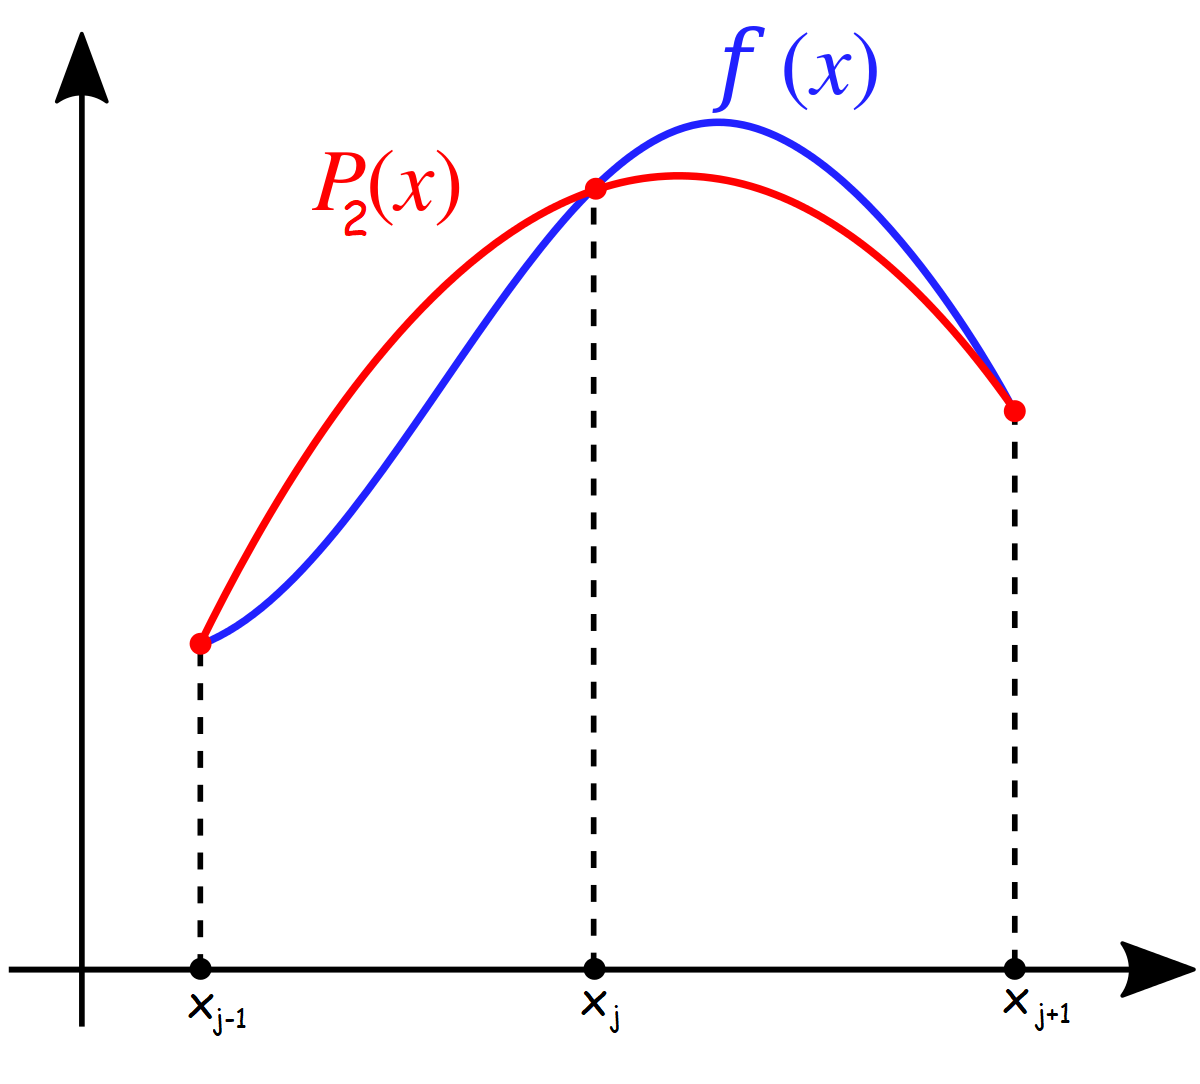
\includegraphics[scale=0.26]{intro}
\end{center}

Esta regla también tiene dos desarrollos en función de la precisión que queramos obtener y en función del número de pasos a ejecutar. Son la Regla de Simpson \textbf{simple} y la \textbf{compuesta}.

\subsubsection{Regla de Simpson simple}

Como explicamos, al aproximar la función por medio de parábolas, usamos el polinomio de interpolación de Lagrange de orden 2 denotado $P_2(x)$.

\begin{center}
$P_2(x)=Ax^2+Bx+C$
\end{center}

Este polinomio nos es de utilidad ya que conocemos el valor de su integral. Así pues, vamos a realizar la siguiente aproximación:

\begin{equation}\label{eq:rss}
\int \limits_{-h}^{h} f(x) \cdot dx \approx 
\int \limits_{-h}^{h} P_2(x) \cdot dx =
\frac{h}{3}(y_0+4y_1+y_2)
\end{equation}

Donde los valores $y_0, y_1, y_2$ corresponden, respectivamente a $f(-h), f(0), f(h)$, que son los puntos por los que hemos hecho pasar la parábola.\\

Podemos ver la aproximación que estamos realizando en el siguiente gráfico:

\begin{center}
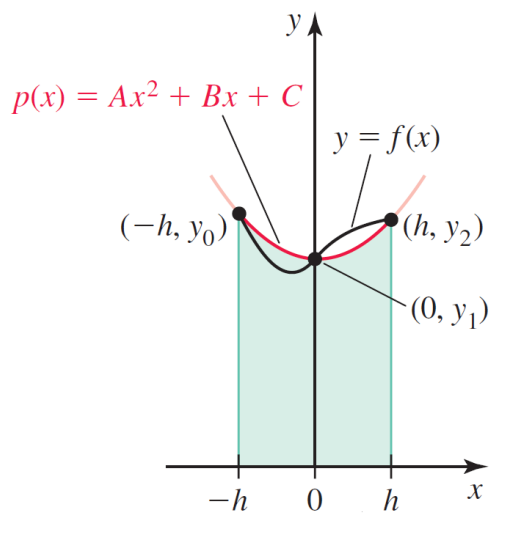
\includegraphics[scale=0.55]{simple}
\end{center}

\underline{\textbf{Demostración de la regla de Simpson simple}} \\

Empezamos viendo el área que encierra la parábola descrita por $P_2(x)$:

\begin{equation}\label{eq:simsim}
\int \limits_{-h}^{h} P_2(x) \cdot dx = 
\int \limits_{-h}^{h} Ax^2+Bx+C \cdot dx =
\frac{2Ah^3}{3}+2Ch = \frac{h}{3}(2Ah^2+6C)
\end{equation}

Como la parábola pasa por los puntos:

\begin{center}
$(-h,y_0)=(-h,f(-h)) \hspace{2mm},\hspace{2mm}
(0,y_1)=(0,f(0)) \hspace{2mm},\hspace{2mm}
(h,y_2)=(h,f(h))$
\end{center}

Entonces:

\begin{equation*}
\left\lbrace
\begin{array}{ll}
\textup y_0 = P_2(-h) = Ah^2-Bh+C\\
\textup y_1 = P_2(0) = C\\
\textup y_2 = P_2(h) = Ah^2+Bh+C\\
\end{array}
\Rightarrow\right.
\end{equation*}

Obteniendo así un sistema de ecuaciones que podemos resolver para A, B y C en función de $y_0$, $y_1$ e $y_2$:

\begin{equation}
\Rightarrow
\left\lbrace
\begin{array}{ll}
\textup C = y_1\\
\textup Ah^2-Bh = y_0 - y_1\\
\textup Ah^2+Bh = y_2 - y_1\\
\textup 2Ah^2 = y_0 + y_2 - 2y_1\\
\end{array}
\right.
\end{equation}

Con estos resultados, podemos sustituir A y C en la ecuación~\ref{eq:simsim}.

\subsubsection{Generalización de la regla de Simpson simple}

Si queremos generalizar la regla para otra región que no necesariamente sea el origen, y si queremos aplicarlo a una función que se extiende por el plano, el primer paso es dividir la parte del dominio de la función que queramos aproximar en un número par \textbf{n} de intervalos. Es decir, hay que dividir el intervalo $[a,b]$ en n subintervalos donde n es un número par. Esto es:

\begin{center}
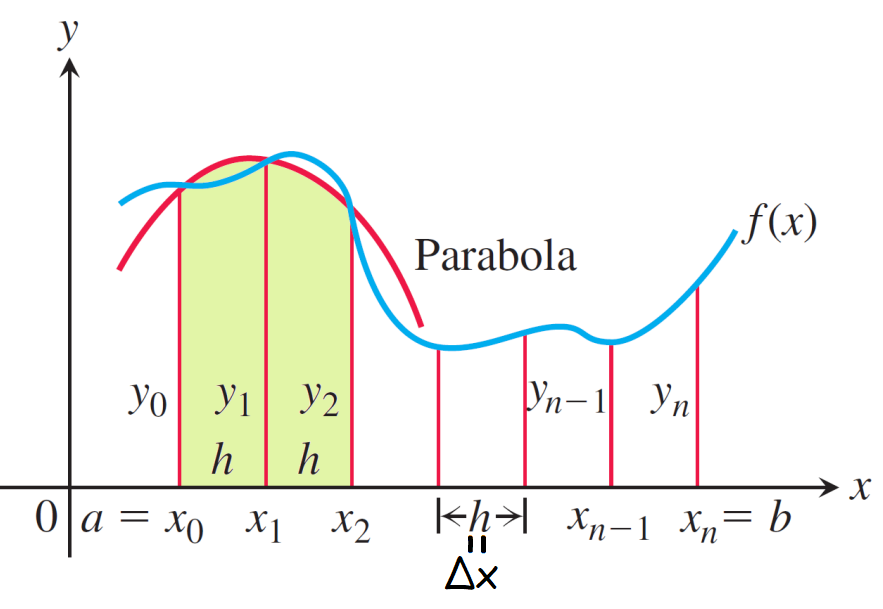
\includegraphics[scale=0.5]{simple_n}
\end{center}

Así, podemos escribir lo siguiente:

\begin{flushleft}
-Las posiciones $x_k$ corresponden a $x_k=a+\Delta x$ con $k=0,1,...,n$.\newline
-La anchura del intervalo, que denominamos paso, es $\Delta x=\frac{b-a}{n}$ .
\end{flushleft}

Con estas aclaraciones y la nueva notación, podemos reescribir la expresión~\ref{eq:rss} de la siguiente forma:

\begin{equation}
\int \limits_{x_{k-1}}^{x_{k+1}} f(x) \cdot dx \approx 
A(P_k) =
\frac{\Delta x}{3}(f(x_{k-1})+4f(x_k)+f(x_{k+1}))
\end{equation}

Por último, debemos observar que como n es par, es decir, $n=2r$, ¡en nuestra aproximación vamos a tener r parábolas!\\

\begin{center}
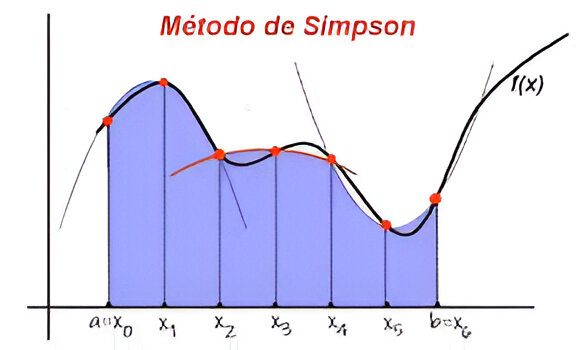
\includegraphics[scale=0.45]{rpara}
\end{center}

En el ejemplo vemos como tenemos 6 intervalos y sin embargo 3 parábolas. \begin{center}($6=2r$)\end{center}

\subsubsection{Regla de Simpson compuesta}

Con estas últimas consideraciones llegamos a la versión compuesta de este método. Básicamente consiste en aplicar la forma general de la versión simple de la regla sucesivas veces hasta cubrir la región finita que queramos aproximar.\\

Esto es lo que acabamos de ver, si dividimos el intervalo finito $[a,b]$ de la función que queremos aproximar en un número par \textbf{n=2r} de subintervalos de longitud $\Delta x=\frac{b-a}{n}$, llegamos a la siguiente expresión:
\begin{equation*}
\int \limits_{a}^{b} f(x) \cdot dx \approx 
\int \sum_{k=1}^{r}A(P_k) =
\frac{\Delta x}{3}\sum_{k=1}^{r}[f(x_{2k-2})+4f(x_{2k-1})+f(x_{2k})] =
\end{equation*}
\begin{equation*}
\;\;\;\;\;\;\;\;\;\;\;\;
=\frac{\Delta x}{3}[f(x_0)+4\sum_{k=1}^{r}f(x_{2k-1})+2\sum_{k=1}^{r-1}f(x_{2k})+f(x_n)] =
\end{equation*}
\begin{equation}
\;\;\;\;\;\;\;\;\;
=\frac{\Delta x}{3}[f(a)+4\sum_{k=1}^{r}f(x_{2k-1})+2\sum_{k=1}^{r-1}f(x_{2k})+f(b)]
\end{equation}

Donde en el penúltimo paso se ha separado $f(x_0)$ ya que para el caso $k=1$, $f(x_{2k-2}=f(x_0)$ al igual que $f(x_n)$ ya que para el caso $k=r$, $f(x_{2k}=f(x_{2r})=f(x_n)$. Además, el último sumatorio está multiplicado por 2 ya que tanto el primer término como el último proporcionan lo mismo para algún valor de k, a excepción de los extremos (pero al sacarlos, nos deshacemos el problema).

\subsubsection{Error de aproximación en la regla de Simpson}

Al igual que en la regla del punto medio, podemos establecer una cota superior para el error cometido al aproximar la integral de una función según el método de Simpson. Para ello, definamos primero el error global en la etapa n.


\begin{equation}
E_n=\left |\displaystyle \int \limits_{a}^{b} f(x) \cdot dx - Sn\right |
\end{equation}

Ahora, sea $S_n$ el resultado de aplicar la regla de Simpson compuesta:
\begin{equation}
S_n = S_{2r} = \frac{\Delta x}{3}
[f(a)+4\sum_{k=1}^{r}f(x_{2k-1})+2\sum_{k=1}^{r-1}f(x_{2k})+f(b)]
\end{equation}

Y sea $K_4 = \smash{\displaystyle\max_{x \in [a,b]}} |f^{(4)}(x)|$. Entonces el error absoluto está acotado por:


\begin{equation}
E_n \leq \frac{K_4(b-a)^5}{180n^4} = \frac{K_4(b-a)}{180}(\Delta x)^4 \sim O((\Delta x)^4)
\end{equation}

Obtenemos como resultado que la magnitud del error es del orden del paso que utilizamos a la cuarta ($O((\Delta x)^4)$). Esto quiere decir, que si f(x) es un polinomio de grado 3 o inferior, ¡la regla de Simpson es exacta!\\

\underline{\textbf{Nota}} \\

El método que acabamos de explicar también es conocido como la regla de Simpson 1/3. Existe otra variante de la regla que es la regla de Simpson 3/8, que difiere de la clásica en que esta usa polinomios de interpolación de Lagrange de 3er orden, además de que la función se tabula con cuatro puntos a igual distancia h formando tres subintervalos. \\

La regla 3/8, comparada en el mismo intervalo que la 1/3, es 2.25 veces más precisa que su compañera. Aún así, en la práctica, rara vez usamos el método 3/8 debido a que el aumento de complejidad es notable (n pasa a tener que ser múltiplo de tres, necesitamos polinomios de grado 3, etc) y debido a que en la mayoría de aplicaciones el método 1/3 nos proporciona la precisión suficiente.\\ 


\section{Soluciones de la Ecuación de Schrödinger}
En esta sección del trabajo nos dedicaremos a obtener las soluciones de la ecuación de Schrödinger de forma numérica y compararlas con las soluciones analíticas de la misma en regiones del espacio donde existen potenciales distintos.

\subsection{Pozo de potencial infinito}

En este primer caso nos encontramos en una región del espacio cubierta por un potencial infinito en toda ella menos en un intervalo finito donde ese potencial tiene un valor de 0 como podemos observar en la siguiente figura:

\begin{figure}[H]
    \centering
    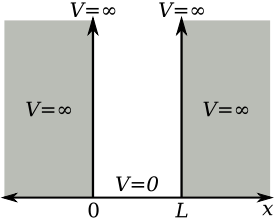
\includegraphics[width=0.5\linewidth]{fotos/particula-caja-wiki.png}
    \caption{Pozo de potencial infinito}
\end{figure}

Una vez planteado el escenario, veamos las funciones de onda que describen a las partículas que nos podemos encontrar aquí y sus niveles de energía correspondientes.

    \subsubsection{Soluciones analíticas}
    Empecemos por hallar sus soluciones analíticas, es decir, las soluciones que obtendríamos si introducimos nuestro potencial junto con el Hamiltoniano en la ecuación de Schrödinger y resolvemos el problema de autovalores y autofunciones bajo estas condiciones.\\

    La solución la podemos escribir según la posición de nuestra partícula:

    \begin{itemize}
        \item \underline{Para x$<$0 y x$>$L}\\
        La función de onda deber ser nula pues para estar en esta región del espacio una partícula necesitaría energía infinita. Por tanto:

        \begin{equation*}
            \psi (x) = 0
        \end{equation*}

        \item \underline{Para 0$<$x$<$L}\\
        Para satisfacer las condiciones de contorno, la función también debe anularse en los extremos del intervalo, esto es:
        
        \begin{equation*}
            \psi (0) = \psi (L) = 0
        \end{equation*}
    
    Con esto definido, en esta región la ecuación de Schrödinger toma la forma: 

    \begin{equation*}
    \frac{d^{2}\psi(x)}{d x^{2}} = -\frac{2m}{\hbar^2} E \psi(x)
    \end{equation*}

    Por lo que ante este problema de Sturm-Liouville se propone la solución correspondiente para resolverlo. El resultado final y por tanto la forma de nuestras soluciones analíticas para cada nivel discreto de energía es:

\begin{equation*}
    \boxed{\psi_n (x) = A\cdot\sin{\left(\frac{n\pi}{a}x\right)}\,\,\,\,\,\,\,\,\,\,\,\, n=1,2,3,...}
\end{equation*}

    donde A es una constante de normalización de valor $A=\sqrt{\frac{2}{a}}$ y $a$ es el límite inferior que delimita el pozo.\\

    Además, los mencionados niveles discretos de energía, que son los autovalores correspondientes a cada autofunción obtenida son los siguientes:

    \begin{equation*}
    \boxed{E_n = \frac{\hbar^2n^2\pi^2}{2ma^2}\,\,\,\,\,\,\,\,\,\,\,\, n=1,2,3,...}
    \end{equation*}

    \end{itemize}

    \subsubsection{Soluciones numéricas}

    El método de obtención de las soluciones numéricas es análogo para las soluciones que siguen. Consiste en realizar una discretización del espacio gracias al método de diferencias finitas y construir el problema de autovalores de forma matricial. Cada solución lleva consigo su propio potencial, lo que modificará la matriz H del Hamiltoniano.\\

    Los autovalores y las autofunciones de esta matriz son las soluciones aproximadas que estamos buscando. Los valores de las autofunciones pueden no estar normalizados, condición necesaria para que lo que estamos estudiando tenga un significado físico, aquí es donde entran los métodos numéricos de integración.\\

    Para normalizar nuestras funciones usaremos tanto el método de los trapecios como el método de Simpson. Con estas funciones ya podremos comparar nuestras soluciones numéricas (aproximadas) con las soluciones analíticas que hemos descrito. La diferencia entre ambas se corresponderá con el error en la aproximación y en la siguiente sección trataremos este tema con detalle.\\
    
    Primero visualicemos lo que hemos explicado para cada solución estudiada en este trabajo. Empecemos por el pozo de potencial infinito:



































    \subsection{Oscilador armónico cuántico}

    \subsection{Pozo de potencial finito}
    \subsection{Características principales}
Un pozo de potencial finito es una de las estrcuturas básicas utilizadas
en física cuántica para observar el comportamiento de la función
de onda de una partícula. Este pozo viene descrito por el siguiente 
potencial:
\begin{equation}
V(x)=\begin{cases} 
    0 & \text{si} \quad -\infty < x \leq -a \\
    -V_0 & \text{si} \quad -a\leq x \leq a \\
    0 & \text{si} \quad a \leq x < \infty \\
 \end{cases}
\end{equation}
Siendo $V_0$ positivo.
Si resolvemos la ecaución de autovalores del Hamiltoniano vamos
a obtener diferentes soluciones en función del tramo en el que 
nos encontremos y dependiendo de si la función es par o impar. Por simplicidad,
vamos a clasificarlas en función de si la solución es par o impar: \\
\par
Si la solución es par obtenemos:
\begin{equation}
    \psi^{(+)}(x)=\begin{cases} 
        C e^{\beta x} & \text{si} \quad -\infty < x \leq -a \\
        A\cos(\alpha x) & \text{si} \quad -a\leq x \leq a \\
        C e^{-\beta x} & \text{si} \quad a \leq x < \infty \\
     \end{cases}
\end{equation}
Por otra parte, si la solución es impar tendremos:
\begin{equation}
    \psi^{(-)}(x)=\begin{cases} 
        -C e^{\beta x} & \text{si} \quad -\infty < x \leq -a \\
        B\sin(\alpha x) & \text{si} \quad -a\leq x \leq a \\
        C e^{-\beta x} & \text{si} \quad a \leq x < \infty \\
     \end{cases}
\end{equation}
Donde A,B y C son las constantes de normalización y $\alpha$ y $\beta$ vienen definidos como: 
$\alpha=\frac{\sqrt{2m(\left\lvert V_0 \right\rvert-\left\lvert E \right\rvert)}}{\hbar}$
; $\beta=\frac{\sqrt{2m\left\lvert E \right\rvert}}{\hbar}$ \\
\par
Como vemos, las constantes de normalización dependen de los 
valores de la energía y de $V_0$. Es decir, variarán según cómo
se haya construido el pozo. En la siguiente sección hablaremos sobre
el pozo que vamos a analizar y el valor de las constantes de normalización.
\begin{figure}[h]
    \centering
    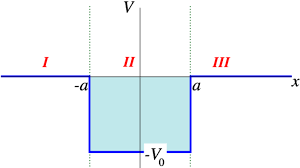
\includegraphics{images.png}
    \caption{Pozo de potencial finito}
    \label{fig:etiqueta}
\end{figure}
\subsection{Construcción del pozo de potencial}
Para este pozo se ha usado el valor para la profundida del pozo
de: $V_0=50$(unidades arbitrarias). Además, como en el ordenador
no podemos incluir el infitio como en la definición formal, hemos 
decidido usar como aproximación en los extremos de análisis $\pm 15$.
Por último, hemos decidido situar el pozo en la región de -5 a 5. \\
\par
Teniendo todo esto en cuenta, hemos obtenido las siguientes constantes
de normalización: $A=B=0,44$ y $C=$. Para ello, hemos usado la definición
de normalización:
\begin{equation}
\int_{a}^{b} \psi^{*}(x) \psi(x) \,dx=1
\end{equation}
Un apunte importante es que para todos los cálculos se ha considerado
que $\hbar=m=1$. \\
\par
A continuación, en las siguiente sección mostraremos las soluciones numéricas 
y las compararemos con las obtenidas analíticamente.
\subsection{Soluciones numéricas}
\subsubsection{Normalización mediante método Simpson}
Las soluciones numéricas han sido obtenidas para un número 
N=1000 puntos y un total de 5 funciones. Las soluciones numéricas
para esas funciones son: 
\begin{figure}[h]
    \centering
    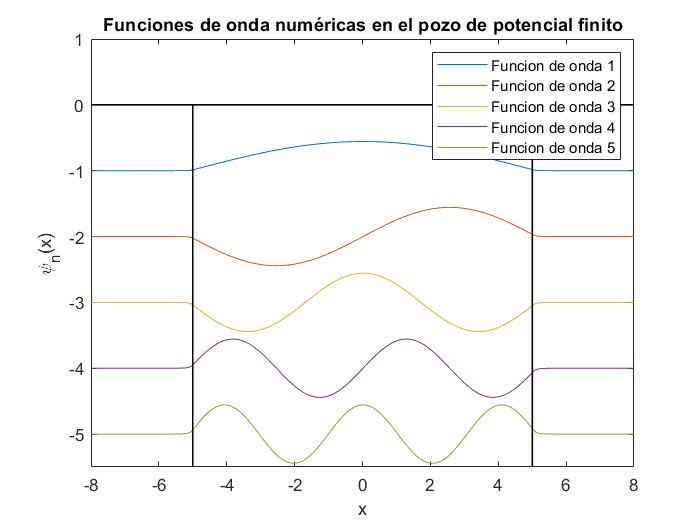
\includegraphics[scale=0.5]{numericas.jpg}
\end{figure} \\
\par
Mientras que las soluciones analíticas son las siguientes:
\newpage
\begin{figure}[h]
    \centering
    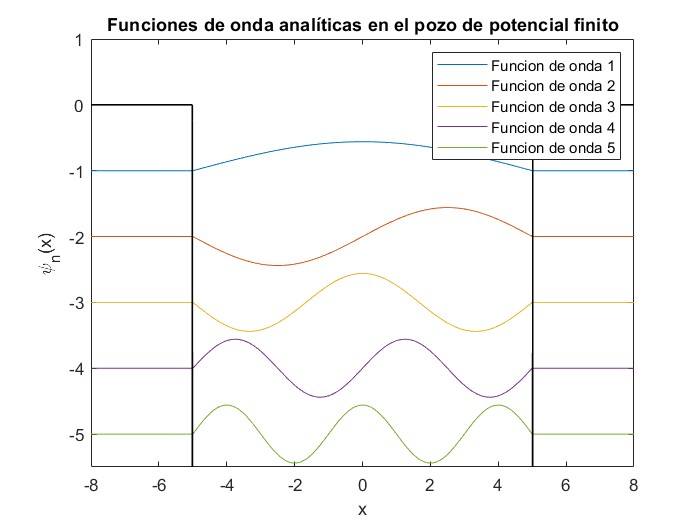
\includegraphics[scale=0.5]{analiticas.jpg}
\end{figure} 
\subsubsection{Normalización mediante método de los trapecios}
De nuevo, se han usado un total de 1000 puntos y un total de 5 
funciones. Mediante este método de normalización se han obtenido
las siguientes soluciones numéricas:
\newpage
\begin{figure}[h]
\centering
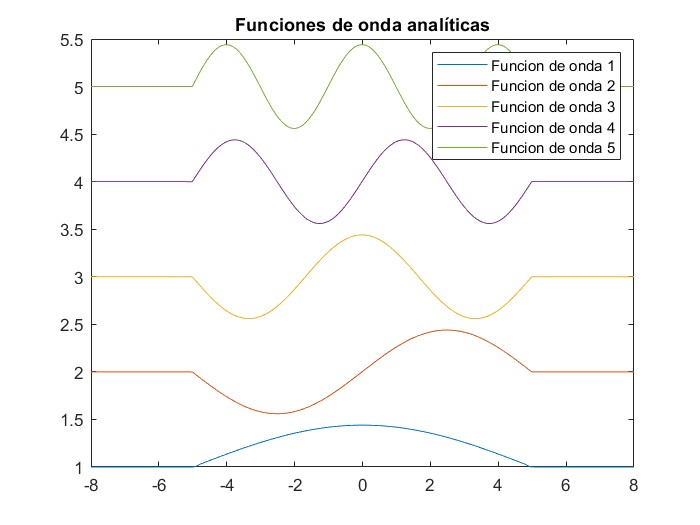
\includegraphics[scale=0.5]{trap.jpg}
\end{figure} 
\section{Estudio de errores para las soluciones obtenidas}

    \subsection{Pozo de potencial infinito}
    
    \subsection{Oscilador armónico cuántico}

    \subsection{Pozo de potencial finito}

    \subsection{Métodos de integración}
    
\section{Consideraciones: Ecuación dependiente del tiempo}

\end{document}
